% TikZ code for Enhanced ReferSAM architecture diagrams
% Usage: Include in LaTeX document with % TikZ code for Enhanced ReferSAM architecture diagrams
% Usage: Include in LaTeX document with % TikZ code for Enhanced ReferSAM architecture diagrams
% Usage: Include in LaTeX document with % TikZ code for Enhanced ReferSAM architecture diagrams
% Usage: Include in LaTeX document with \input{tikz_architecture.tex}
% Requires: \usepackage{tikz} \usetikzlibrary{shapes,arrows,positioning,calc}

\documentclass[tikz,border=2mm]{standalone}
\usepackage{tikz}
\usetikzlibrary{shapes,arrows,positioning,calc,decorations.pathreplacing}

% Color definitions (professional scheme)
\definecolor{inputcolor}{RGB}{227,242,253}
\definecolor{encodercolor}{RGB}{255,243,224}
\definecolor{adaptercolor}{RGB}{232,245,233}
\definecolor{fusioncolor}{RGB}{243,229,245}
\definecolor{decodercolor}{RGB}{252,228,236}
\definecolor{outputcolor}{RGB}{255,249,196}
\definecolor{losscolor}{RGB}{255,235,238}
\definecolor{textcolor}{RGB}{224,242,241}
\definecolor{enhancedcolor}{RGB}{197,225,165}
\definecolor{bordercolor}{RGB}{66,66,66}
\definecolor{arrowcolor}{RGB}{25,118,210}
\definecolor{highlightcolor}{RGB}{211,47,47}

\tikzset{
    module/.style={
        rectangle,
        rounded corners=3pt,
        minimum width=2.5cm,
        minimum height=1cm,
        text centered,
        draw=bordercolor,
        line width=1.5pt,
        font=\small\bfseries
    },
    inputmodule/.style={module, fill=inputcolor},
    encodermodule/.style={module, fill=encodercolor},
    adaptermodule/.style={module, fill=adaptercolor},
    fusionmodule/.style={module, fill=fusioncolor},
    decodermodule/.style={module, fill=decodercolor},
    outputmodule/.style={module, fill=outputcolor},
    lossmodule/.style={module, fill=losscolor},
    textmodule/.style={module, fill=textcolor},
    enhancedmodule/.style={module, fill=enhancedcolor, draw=highlightcolor, line width=2pt},
    arrow/.style={->, >=stealth, line width=2pt, color=arrowcolor}
}

\begin{document}

% Overall Architecture
\begin{tikzpicture}[node distance=1.5cm and 2cm]
    % Title
    \node[font=\Large\bfseries] (title) at (9,10.5) {Enhanced ReferSAM Architecture};
    
    % Input layer
    \node[inputmodule] (image) at (2.25,9) {Image\\[B$\times$3$\times$H$\times$W]};
    \node[textmodule] (text) at (2.25,7.3) {Text\\[B$\times$N]};
    
    % Encoders
    \node[encodermodule] (vit) at (5.75,9) {ViT Image\\Encoder};
    \node[encodermodule] (textenc) at (5.75,7.3) {Text\\Encoder};
    
    % ViT Adapter (main container)
    \node[adaptermodule, minimum width=4.5cm, minimum height=3.5cm, 
          fill=adaptercolor!30, draw=bordercolor, line width=2pt] (adapter) at (10.25,7.5) {};
    \node[font=\large\bfseries] (adaptertitle) at (10.25,9.2) {ViT Adapter (Enhanced)};
    
    % Enhanced modules inside adapter
    \node[enhancedmodule, minimum width=3.5cm, minimum height=0.8cm] 
          (msf) at (10.25,8.4) {MultiScale Fusion};
    \node[enhancedmodule, minimum width=3.5cm, minimum height=0.8cm] 
          (c1c2) at (10.25,7.4) {Enhanced C1C2 Fusion};
    \node[enhancedmodule, minimum width=3.5cm, minimum height=0.8cm] 
          (textattn) at (10.25,6.4) {Text Attention Aggregation};
    
    % Features
    \node[adaptermodule] (feat) at (14.75,7.6) {Adapter\\Features};
    \node[decodermodule] (maskfeat) at (14.75,5.8) {Mask Feature\\\& Prompts};
    \node[decodermodule] (decoder) at (14.75,3.5) {SAM Mask\\Decoder};
    \node[outputmodule] (output) at (14.75,1.5) {Predicted\\Mask};
    
    % Loss
    \node[lossmodule, minimum height=2cm, draw=highlightcolor, line width=2pt] 
          (loss) at (2.5,4) {Enhanced Loss\\Functions\\(Focal+IoU+Boundary)};
    
    % Arrows
    \draw[arrow] (image) -- (vit);
    \draw[arrow] (text) -- (textenc);
    \draw[arrow] (vit) -- (adapter);
    \draw[arrow] (textenc) -- (adapter);
    \draw[arrow] (adapter) -- (feat);
    \draw[arrow] (feat) -- (maskfeat);
    \draw[arrow] (maskfeat) -- (decoder);
    \draw[arrow] (decoder) -- (output);
    \draw[arrow, dashed, color=highlightcolor] (output) to[out=180,in=0] (loss);
    \node[font=\small\itshape, color=highlightcolor] at (8.5,1.5) {Training Loss};
\end{tikzpicture}

% MultiScale Fusion Module
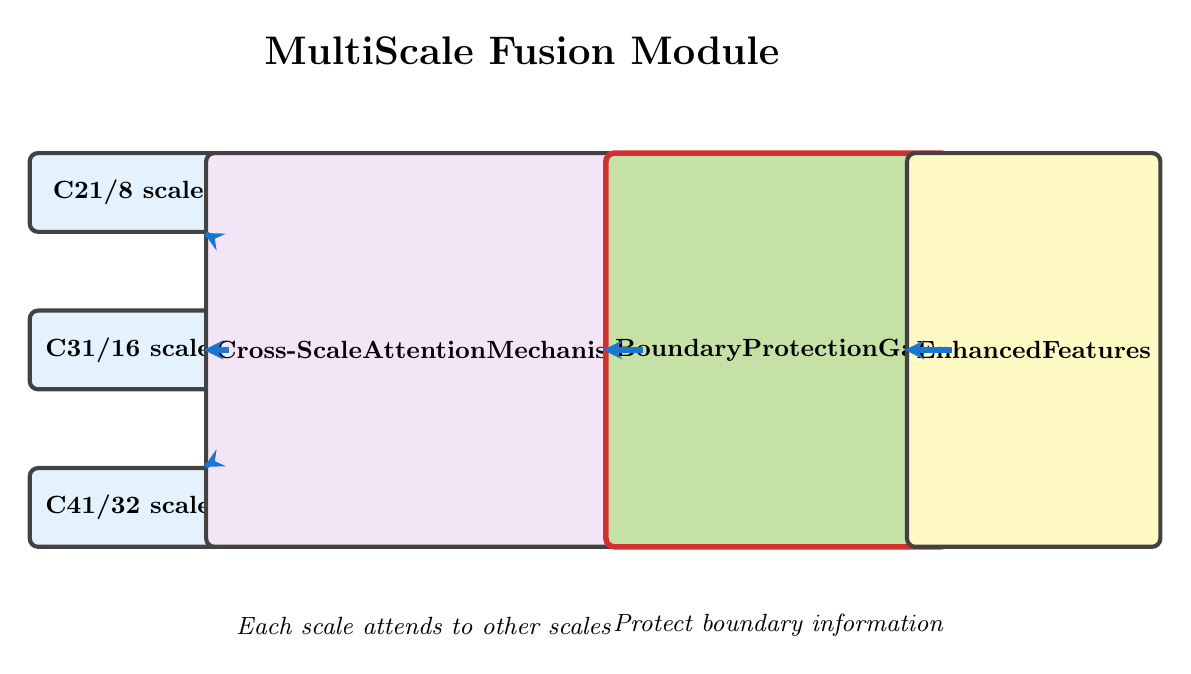
\begin{tikzpicture}[node distance=1.5cm and 2cm]
    \node[font=\Large\bfseries] (title) at (7,8.3) {MultiScale Fusion Module};
    
    % Input features
    \node[inputmodule] (c2) at (2,6.5) {C2\\1/8 scale};
    \node[inputmodule] (c3) at (2,4.5) {C3\\1/16 scale};
    \node[inputmodule] (c4) at (2,2.5) {C4\\1/32 scale};
    
    % Processing modules
    \node[fusionmodule, minimum height=5cm] (attn) at (5.75,4.5) 
          {Cross-Scale\\Attention\\Mechanism};
    \node[enhancedmodule, minimum height=5cm] (gate) at (10.25,4.5) 
          {Boundary\\Protection\\Gate};
    
    % Output
    \node[outputmodule, minimum height=5cm, minimum width=0.8cm] (out) at (13.5,4.5) 
          {Enhanced\\Features};
    
    % Arrows
    \draw[arrow] (c2) -- (attn);
    \draw[arrow] (c3) -- (attn);
    \draw[arrow] (c4) -- (attn);
    \draw[arrow] (attn) -- (gate);
    \draw[arrow] (gate) -- (out);
    
    % Annotations
    \node[font=\small\itshape] at (5.75,1) {Each scale attends to other scales};
    \node[font=\small\itshape] at (10.25,1) {Protect boundary information};
\end{tikzpicture}

% Enhanced C1C2 Fusion Module
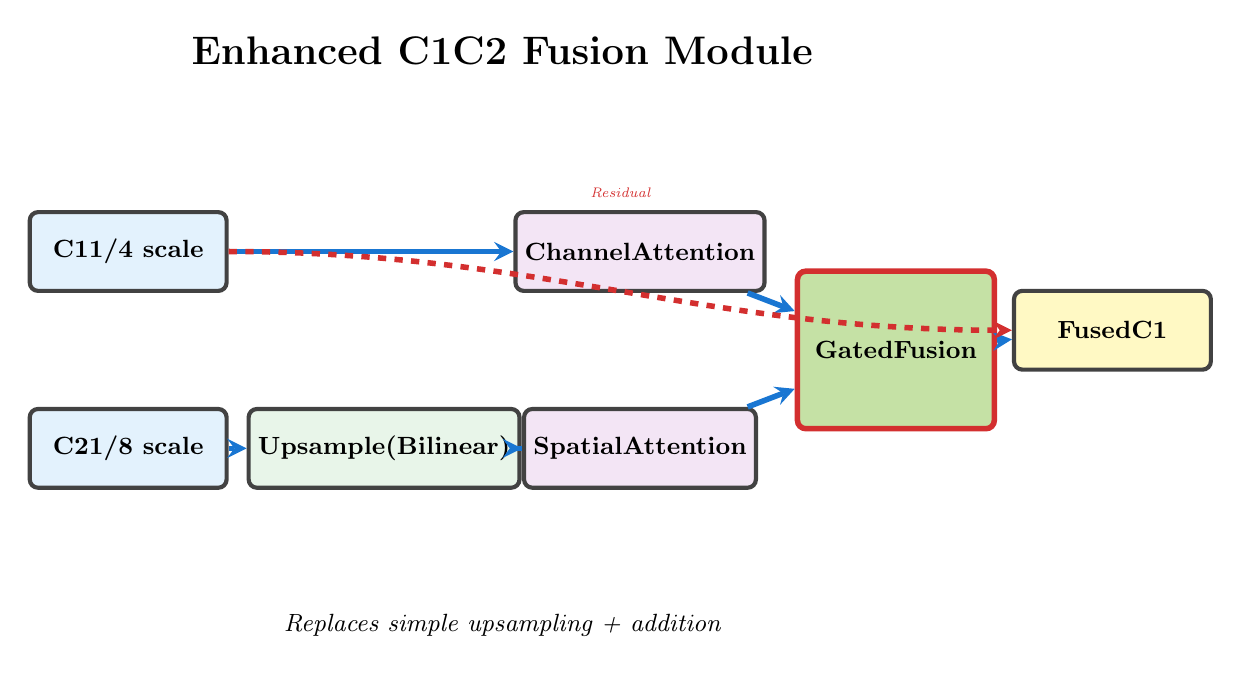
\begin{tikzpicture}[node distance=1.5cm and 2cm]
    \node[font=\Large\bfseries] (title) at (7,8.3) {Enhanced C1C2 Fusion Module};
    
    % Input
    \node[inputmodule] (c1) at (2.25,5.75) {C1\\1/4 scale};
    \node[inputmodule] (c2) at (2.25,3.25) {C2\\1/8 scale};
    
    % Upsample
    \node[adaptermodule] (upsample) at (5.5,3.25) {Upsample\\(Bilinear)};
    
    % Attention
    \node[fusionmodule] (chattn) at (8.75,5.75) {Channel\\Attention};
    \node[fusionmodule] (spattn) at (8.75,3.25) {Spatial\\Attention};
    
    % Gate
    \node[enhancedmodule, minimum height=2cm] (gate) at (12,4.5) {Gated\\Fusion};
    
    % Output
    \node[outputmodule] (out) at (14.75,4.75) {Fused\\C1};
    
    % Arrows
    \draw[arrow] (c1) -- (chattn);
    \draw[arrow] (c2) -- (upsample);
    \draw[arrow] (upsample) -- (spattn);
    \draw[arrow] (chattn) -- (gate);
    \draw[arrow] (spattn) -- (gate);
    \draw[arrow] (gate) -- (out);
    \draw[arrow, dashed, color=highlightcolor] (c1) to[out=0,in=180] (out);
    \node[font=\tiny\itshape, color=highlightcolor] at (8.5,6.5) {Residual};
    
    \node[font=\small\itshape] at (7,1) {Replaces simple upsampling + addition};
\end{tikzpicture}

% Text Attention Aggregation Module
\begin{tikzpicture}[node distance=1.5cm and 2cm]
    \node[font=\Large\bfseries] (title) at (7,8.3) {Text Attention Aggregation Module};
    
    % Input
    \node[textmodule, minimum height=2.5cm] (text) at (2.25,5.75) {Text Features\\[B$\times$N$\times$D]};
    
    % Processing
    \node[inputmodule] (base) at (5.75,6.6) {Base Token\\(EOS/CLS)};
    \node[fusionmodule] (attn) at (5.75,4.75) {Multi-Head\\Attention};
    \node[enhancedmodule] (query) at (5.75,2.25) {Learnable\\Query};
    
    % Fusion
    \node[enhancedmodule, minimum height=2.5cm] (fusion) at (9.5,4.75) {Weighted\\Fusion\\(Learnable)};
    
    % Output
    \node[outputmodule] (out) at (12.75,4.75) {Aggregated\\Text Feature};
    
    % Arrows
    \draw[arrow] (text) -- (base);
    \draw[arrow] (text) -- (attn);
    \draw[arrow] (query) -- (attn);
    \draw[arrow] (base) -- (fusion);
    \draw[arrow] (attn) -- (fusion);
    \draw[arrow] (fusion) -- (out);
    
    \node[font=\small\itshape] at (7,1) {Replaces simple token selection (EOS/CLS)};
\end{tikzpicture}

% Enhanced Loss Functions Module
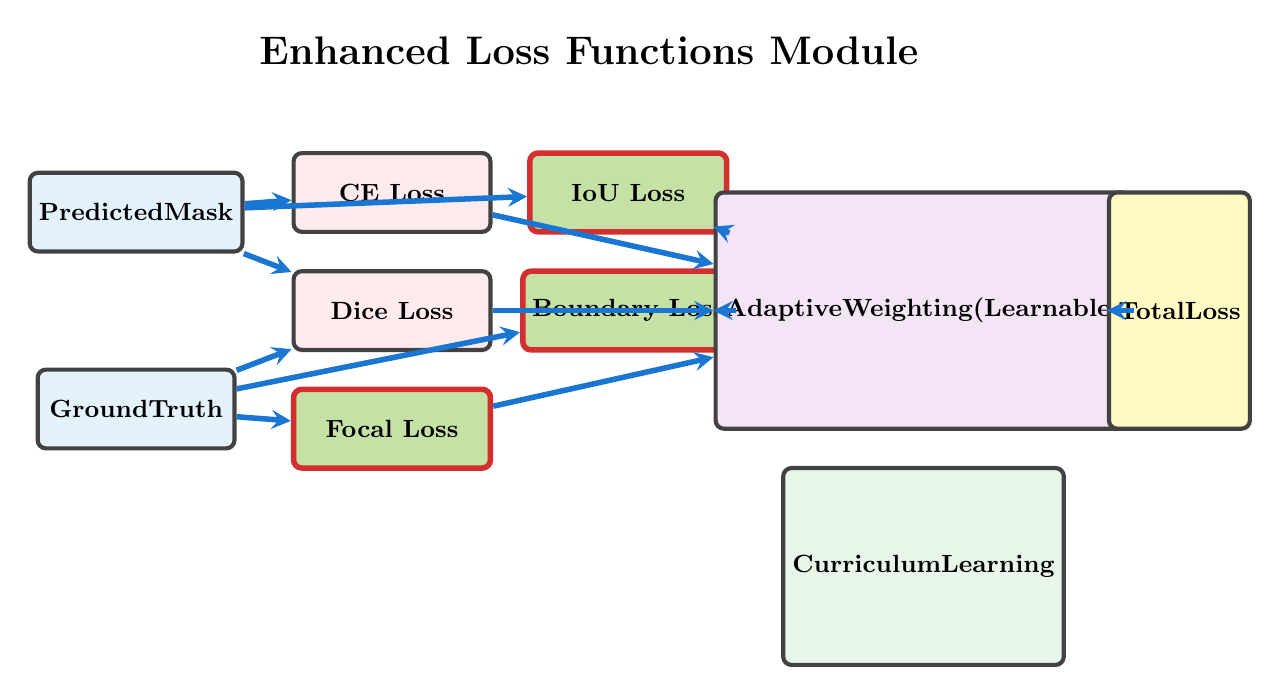
\begin{tikzpicture}[node distance=1.5cm and 2cm]
    \node[font=\Large\bfseries] (title) at (8,8.3) {Enhanced Loss Functions Module};
    
    % Input
    \node[inputmodule] (pred) at (2.25,6.25) {Predicted\\Mask};
    \node[inputmodule] (target) at (2.25,3.75) {Ground\\Truth};
    
    % Loss functions
    \node[lossmodule] (ce) at (5.5,6.5) {CE Loss};
    \node[lossmodule] (dice) at (5.5,5) {Dice Loss};
    \node[enhancedmodule] (focal) at (5.5,3.5) {Focal Loss};
    \node[enhancedmodule] (iou) at (8.5,6.5) {IoU Loss};
    \node[enhancedmodule] (boundary) at (8.5,5) {Boundary Loss};
    
    % Adaptive weighting
    \node[fusionmodule, minimum height=3cm] (adaptive) at (12.25,5) {Adaptive\\Weighting\\(Learnable)};
    
    % Curriculum learning
    \node[adaptermodule, minimum height=2.5cm] (curriculum) at (12.25,1.75) {Curriculum\\Learning};
    
    % Total loss
    \node[outputmodule, minimum height=3cm, minimum width=1cm] (total) at (15.5,5) {Total\\Loss};
    
    % Arrows
    \draw[arrow] (pred) -- (ce);
    \draw[arrow] (pred) -- (dice);
    \draw[arrow] (target) -- (focal);
    \draw[arrow] (target) -- (dice);
    \draw[arrow] (pred) -- (iou);
    \draw[arrow] (target) -- (boundary);
    \draw[arrow] (ce) -- (adaptive);
    \draw[arrow] (dice) -- (adaptive);
    \draw[arrow] (focal) -- (adaptive);
    \draw[arrow] (iou) -- (adaptive);
    \draw[arrow] (boundary) -- (adaptive);
    \draw[arrow] (adaptive) -- (total);
\end{tikzpicture}

\end{document}


% Requires: \usepackage{tikz} \usetikzlibrary{shapes,arrows,positioning,calc}

\documentclass[tikz,border=2mm]{standalone}
\usepackage{tikz}
\usetikzlibrary{shapes,arrows,positioning,calc,decorations.pathreplacing}

% Color definitions (professional scheme)
\definecolor{inputcolor}{RGB}{227,242,253}
\definecolor{encodercolor}{RGB}{255,243,224}
\definecolor{adaptercolor}{RGB}{232,245,233}
\definecolor{fusioncolor}{RGB}{243,229,245}
\definecolor{decodercolor}{RGB}{252,228,236}
\definecolor{outputcolor}{RGB}{255,249,196}
\definecolor{losscolor}{RGB}{255,235,238}
\definecolor{textcolor}{RGB}{224,242,241}
\definecolor{enhancedcolor}{RGB}{197,225,165}
\definecolor{bordercolor}{RGB}{66,66,66}
\definecolor{arrowcolor}{RGB}{25,118,210}
\definecolor{highlightcolor}{RGB}{211,47,47}

\tikzset{
    module/.style={
        rectangle,
        rounded corners=3pt,
        minimum width=2.5cm,
        minimum height=1cm,
        text centered,
        draw=bordercolor,
        line width=1.5pt,
        font=\small\bfseries
    },
    inputmodule/.style={module, fill=inputcolor},
    encodermodule/.style={module, fill=encodercolor},
    adaptermodule/.style={module, fill=adaptercolor},
    fusionmodule/.style={module, fill=fusioncolor},
    decodermodule/.style={module, fill=decodercolor},
    outputmodule/.style={module, fill=outputcolor},
    lossmodule/.style={module, fill=losscolor},
    textmodule/.style={module, fill=textcolor},
    enhancedmodule/.style={module, fill=enhancedcolor, draw=highlightcolor, line width=2pt},
    arrow/.style={->, >=stealth, line width=2pt, color=arrowcolor}
}

\begin{document}

% Overall Architecture
\begin{tikzpicture}[node distance=1.5cm and 2cm]
    % Title
    \node[font=\Large\bfseries] (title) at (9,10.5) {Enhanced ReferSAM Architecture};
    
    % Input layer
    \node[inputmodule] (image) at (2.25,9) {Image\\[B$\times$3$\times$H$\times$W]};
    \node[textmodule] (text) at (2.25,7.3) {Text\\[B$\times$N]};
    
    % Encoders
    \node[encodermodule] (vit) at (5.75,9) {ViT Image\\Encoder};
    \node[encodermodule] (textenc) at (5.75,7.3) {Text\\Encoder};
    
    % ViT Adapter (main container)
    \node[adaptermodule, minimum width=4.5cm, minimum height=3.5cm, 
          fill=adaptercolor!30, draw=bordercolor, line width=2pt] (adapter) at (10.25,7.5) {};
    \node[font=\large\bfseries] (adaptertitle) at (10.25,9.2) {ViT Adapter (Enhanced)};
    
    % Enhanced modules inside adapter
    \node[enhancedmodule, minimum width=3.5cm, minimum height=0.8cm] 
          (msf) at (10.25,8.4) {MultiScale Fusion};
    \node[enhancedmodule, minimum width=3.5cm, minimum height=0.8cm] 
          (c1c2) at (10.25,7.4) {Enhanced C1C2 Fusion};
    \node[enhancedmodule, minimum width=3.5cm, minimum height=0.8cm] 
          (textattn) at (10.25,6.4) {Text Attention Aggregation};
    
    % Features
    \node[adaptermodule] (feat) at (14.75,7.6) {Adapter\\Features};
    \node[decodermodule] (maskfeat) at (14.75,5.8) {Mask Feature\\\& Prompts};
    \node[decodermodule] (decoder) at (14.75,3.5) {SAM Mask\\Decoder};
    \node[outputmodule] (output) at (14.75,1.5) {Predicted\\Mask};
    
    % Loss
    \node[lossmodule, minimum height=2cm, draw=highlightcolor, line width=2pt] 
          (loss) at (2.5,4) {Enhanced Loss\\Functions\\(Focal+IoU+Boundary)};
    
    % Arrows
    \draw[arrow] (image) -- (vit);
    \draw[arrow] (text) -- (textenc);
    \draw[arrow] (vit) -- (adapter);
    \draw[arrow] (textenc) -- (adapter);
    \draw[arrow] (adapter) -- (feat);
    \draw[arrow] (feat) -- (maskfeat);
    \draw[arrow] (maskfeat) -- (decoder);
    \draw[arrow] (decoder) -- (output);
    \draw[arrow, dashed, color=highlightcolor] (output) to[out=180,in=0] (loss);
    \node[font=\small\itshape, color=highlightcolor] at (8.5,1.5) {Training Loss};
\end{tikzpicture}

% MultiScale Fusion Module
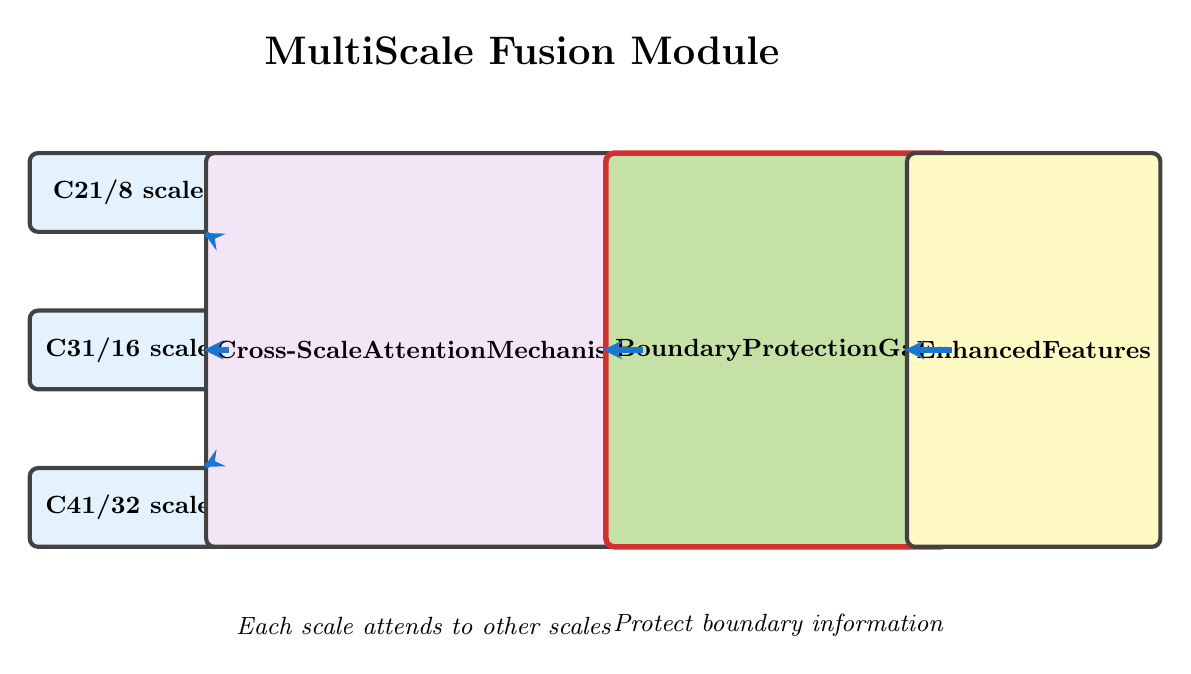
\begin{tikzpicture}[node distance=1.5cm and 2cm]
    \node[font=\Large\bfseries] (title) at (7,8.3) {MultiScale Fusion Module};
    
    % Input features
    \node[inputmodule] (c2) at (2,6.5) {C2\\1/8 scale};
    \node[inputmodule] (c3) at (2,4.5) {C3\\1/16 scale};
    \node[inputmodule] (c4) at (2,2.5) {C4\\1/32 scale};
    
    % Processing modules
    \node[fusionmodule, minimum height=5cm] (attn) at (5.75,4.5) 
          {Cross-Scale\\Attention\\Mechanism};
    \node[enhancedmodule, minimum height=5cm] (gate) at (10.25,4.5) 
          {Boundary\\Protection\\Gate};
    
    % Output
    \node[outputmodule, minimum height=5cm, minimum width=0.8cm] (out) at (13.5,4.5) 
          {Enhanced\\Features};
    
    % Arrows
    \draw[arrow] (c2) -- (attn);
    \draw[arrow] (c3) -- (attn);
    \draw[arrow] (c4) -- (attn);
    \draw[arrow] (attn) -- (gate);
    \draw[arrow] (gate) -- (out);
    
    % Annotations
    \node[font=\small\itshape] at (5.75,1) {Each scale attends to other scales};
    \node[font=\small\itshape] at (10.25,1) {Protect boundary information};
\end{tikzpicture}

% Enhanced C1C2 Fusion Module
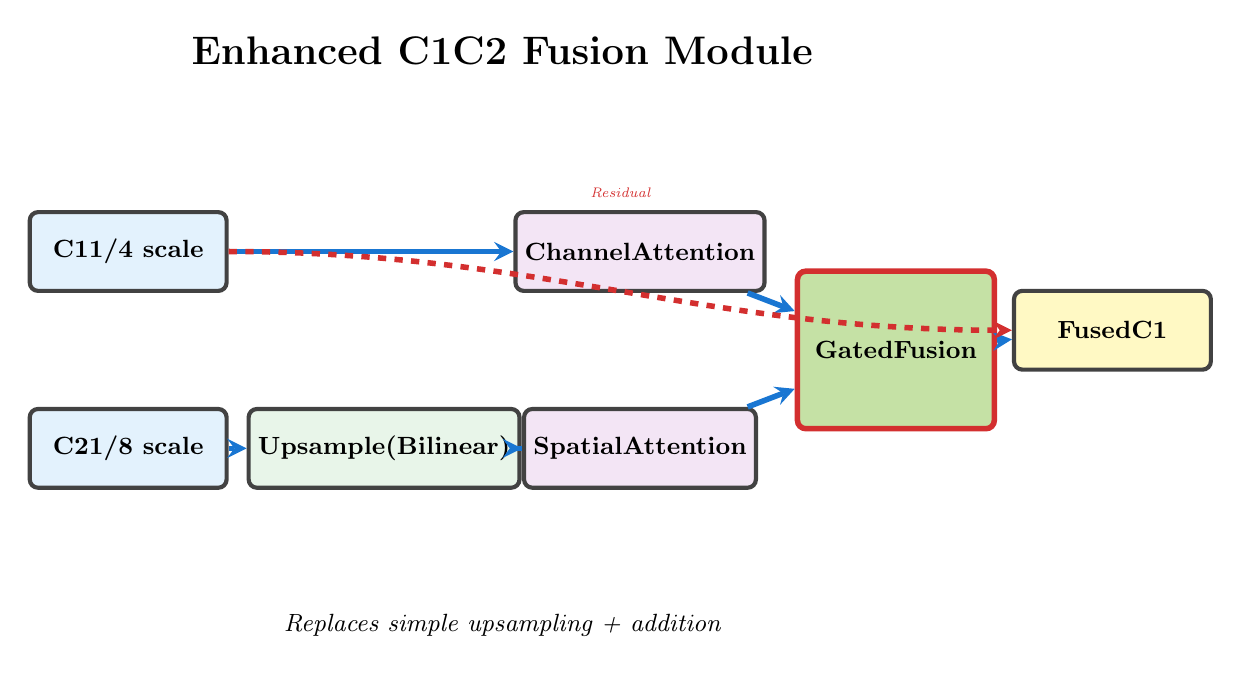
\begin{tikzpicture}[node distance=1.5cm and 2cm]
    \node[font=\Large\bfseries] (title) at (7,8.3) {Enhanced C1C2 Fusion Module};
    
    % Input
    \node[inputmodule] (c1) at (2.25,5.75) {C1\\1/4 scale};
    \node[inputmodule] (c2) at (2.25,3.25) {C2\\1/8 scale};
    
    % Upsample
    \node[adaptermodule] (upsample) at (5.5,3.25) {Upsample\\(Bilinear)};
    
    % Attention
    \node[fusionmodule] (chattn) at (8.75,5.75) {Channel\\Attention};
    \node[fusionmodule] (spattn) at (8.75,3.25) {Spatial\\Attention};
    
    % Gate
    \node[enhancedmodule, minimum height=2cm] (gate) at (12,4.5) {Gated\\Fusion};
    
    % Output
    \node[outputmodule] (out) at (14.75,4.75) {Fused\\C1};
    
    % Arrows
    \draw[arrow] (c1) -- (chattn);
    \draw[arrow] (c2) -- (upsample);
    \draw[arrow] (upsample) -- (spattn);
    \draw[arrow] (chattn) -- (gate);
    \draw[arrow] (spattn) -- (gate);
    \draw[arrow] (gate) -- (out);
    \draw[arrow, dashed, color=highlightcolor] (c1) to[out=0,in=180] (out);
    \node[font=\tiny\itshape, color=highlightcolor] at (8.5,6.5) {Residual};
    
    \node[font=\small\itshape] at (7,1) {Replaces simple upsampling + addition};
\end{tikzpicture}

% Text Attention Aggregation Module
\begin{tikzpicture}[node distance=1.5cm and 2cm]
    \node[font=\Large\bfseries] (title) at (7,8.3) {Text Attention Aggregation Module};
    
    % Input
    \node[textmodule, minimum height=2.5cm] (text) at (2.25,5.75) {Text Features\\[B$\times$N$\times$D]};
    
    % Processing
    \node[inputmodule] (base) at (5.75,6.6) {Base Token\\(EOS/CLS)};
    \node[fusionmodule] (attn) at (5.75,4.75) {Multi-Head\\Attention};
    \node[enhancedmodule] (query) at (5.75,2.25) {Learnable\\Query};
    
    % Fusion
    \node[enhancedmodule, minimum height=2.5cm] (fusion) at (9.5,4.75) {Weighted\\Fusion\\(Learnable)};
    
    % Output
    \node[outputmodule] (out) at (12.75,4.75) {Aggregated\\Text Feature};
    
    % Arrows
    \draw[arrow] (text) -- (base);
    \draw[arrow] (text) -- (attn);
    \draw[arrow] (query) -- (attn);
    \draw[arrow] (base) -- (fusion);
    \draw[arrow] (attn) -- (fusion);
    \draw[arrow] (fusion) -- (out);
    
    \node[font=\small\itshape] at (7,1) {Replaces simple token selection (EOS/CLS)};
\end{tikzpicture}

% Enhanced Loss Functions Module
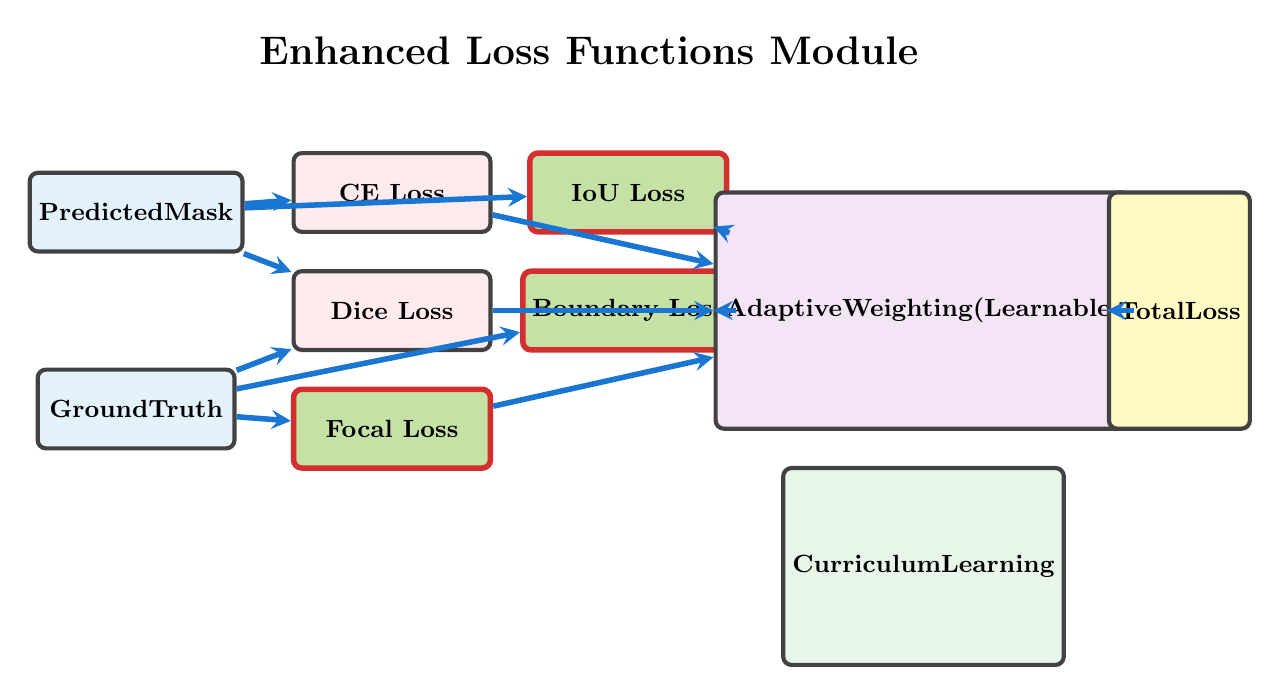
\begin{tikzpicture}[node distance=1.5cm and 2cm]
    \node[font=\Large\bfseries] (title) at (8,8.3) {Enhanced Loss Functions Module};
    
    % Input
    \node[inputmodule] (pred) at (2.25,6.25) {Predicted\\Mask};
    \node[inputmodule] (target) at (2.25,3.75) {Ground\\Truth};
    
    % Loss functions
    \node[lossmodule] (ce) at (5.5,6.5) {CE Loss};
    \node[lossmodule] (dice) at (5.5,5) {Dice Loss};
    \node[enhancedmodule] (focal) at (5.5,3.5) {Focal Loss};
    \node[enhancedmodule] (iou) at (8.5,6.5) {IoU Loss};
    \node[enhancedmodule] (boundary) at (8.5,5) {Boundary Loss};
    
    % Adaptive weighting
    \node[fusionmodule, minimum height=3cm] (adaptive) at (12.25,5) {Adaptive\\Weighting\\(Learnable)};
    
    % Curriculum learning
    \node[adaptermodule, minimum height=2.5cm] (curriculum) at (12.25,1.75) {Curriculum\\Learning};
    
    % Total loss
    \node[outputmodule, minimum height=3cm, minimum width=1cm] (total) at (15.5,5) {Total\\Loss};
    
    % Arrows
    \draw[arrow] (pred) -- (ce);
    \draw[arrow] (pred) -- (dice);
    \draw[arrow] (target) -- (focal);
    \draw[arrow] (target) -- (dice);
    \draw[arrow] (pred) -- (iou);
    \draw[arrow] (target) -- (boundary);
    \draw[arrow] (ce) -- (adaptive);
    \draw[arrow] (dice) -- (adaptive);
    \draw[arrow] (focal) -- (adaptive);
    \draw[arrow] (iou) -- (adaptive);
    \draw[arrow] (boundary) -- (adaptive);
    \draw[arrow] (adaptive) -- (total);
\end{tikzpicture}

\end{document}


% Requires: \usepackage{tikz} \usetikzlibrary{shapes,arrows,positioning,calc}

\documentclass[tikz,border=2mm]{standalone}
\usepackage{tikz}
\usetikzlibrary{shapes,arrows,positioning,calc,decorations.pathreplacing}

% Color definitions (professional scheme)
\definecolor{inputcolor}{RGB}{227,242,253}
\definecolor{encodercolor}{RGB}{255,243,224}
\definecolor{adaptercolor}{RGB}{232,245,233}
\definecolor{fusioncolor}{RGB}{243,229,245}
\definecolor{decodercolor}{RGB}{252,228,236}
\definecolor{outputcolor}{RGB}{255,249,196}
\definecolor{losscolor}{RGB}{255,235,238}
\definecolor{textcolor}{RGB}{224,242,241}
\definecolor{enhancedcolor}{RGB}{197,225,165}
\definecolor{bordercolor}{RGB}{66,66,66}
\definecolor{arrowcolor}{RGB}{25,118,210}
\definecolor{highlightcolor}{RGB}{211,47,47}

\tikzset{
    module/.style={
        rectangle,
        rounded corners=3pt,
        minimum width=2.5cm,
        minimum height=1cm,
        text centered,
        draw=bordercolor,
        line width=1.5pt,
        font=\small\bfseries
    },
    inputmodule/.style={module, fill=inputcolor},
    encodermodule/.style={module, fill=encodercolor},
    adaptermodule/.style={module, fill=adaptercolor},
    fusionmodule/.style={module, fill=fusioncolor},
    decodermodule/.style={module, fill=decodercolor},
    outputmodule/.style={module, fill=outputcolor},
    lossmodule/.style={module, fill=losscolor},
    textmodule/.style={module, fill=textcolor},
    enhancedmodule/.style={module, fill=enhancedcolor, draw=highlightcolor, line width=2pt},
    arrow/.style={->, >=stealth, line width=2pt, color=arrowcolor}
}

\begin{document}

% Overall Architecture
\begin{tikzpicture}[node distance=1.5cm and 2cm]
    % Title
    \node[font=\Large\bfseries] (title) at (9,10.5) {Enhanced ReferSAM Architecture};
    
    % Input layer
    \node[inputmodule] (image) at (2.25,9) {Image\\[B$\times$3$\times$H$\times$W]};
    \node[textmodule] (text) at (2.25,7.3) {Text\\[B$\times$N]};
    
    % Encoders
    \node[encodermodule] (vit) at (5.75,9) {ViT Image\\Encoder};
    \node[encodermodule] (textenc) at (5.75,7.3) {Text\\Encoder};
    
    % ViT Adapter (main container)
    \node[adaptermodule, minimum width=4.5cm, minimum height=3.5cm, 
          fill=adaptercolor!30, draw=bordercolor, line width=2pt] (adapter) at (10.25,7.5) {};
    \node[font=\large\bfseries] (adaptertitle) at (10.25,9.2) {ViT Adapter (Enhanced)};
    
    % Enhanced modules inside adapter
    \node[enhancedmodule, minimum width=3.5cm, minimum height=0.8cm] 
          (msf) at (10.25,8.4) {MultiScale Fusion};
    \node[enhancedmodule, minimum width=3.5cm, minimum height=0.8cm] 
          (c1c2) at (10.25,7.4) {Enhanced C1C2 Fusion};
    \node[enhancedmodule, minimum width=3.5cm, minimum height=0.8cm] 
          (textattn) at (10.25,6.4) {Text Attention Aggregation};
    
    % Features
    \node[adaptermodule] (feat) at (14.75,7.6) {Adapter\\Features};
    \node[decodermodule] (maskfeat) at (14.75,5.8) {Mask Feature\\\& Prompts};
    \node[decodermodule] (decoder) at (14.75,3.5) {SAM Mask\\Decoder};
    \node[outputmodule] (output) at (14.75,1.5) {Predicted\\Mask};
    
    % Loss
    \node[lossmodule, minimum height=2cm, draw=highlightcolor, line width=2pt] 
          (loss) at (2.5,4) {Enhanced Loss\\Functions\\(Focal+IoU+Boundary)};
    
    % Arrows
    \draw[arrow] (image) -- (vit);
    \draw[arrow] (text) -- (textenc);
    \draw[arrow] (vit) -- (adapter);
    \draw[arrow] (textenc) -- (adapter);
    \draw[arrow] (adapter) -- (feat);
    \draw[arrow] (feat) -- (maskfeat);
    \draw[arrow] (maskfeat) -- (decoder);
    \draw[arrow] (decoder) -- (output);
    \draw[arrow, dashed, color=highlightcolor] (output) to[out=180,in=0] (loss);
    \node[font=\small\itshape, color=highlightcolor] at (8.5,1.5) {Training Loss};
\end{tikzpicture}

% MultiScale Fusion Module
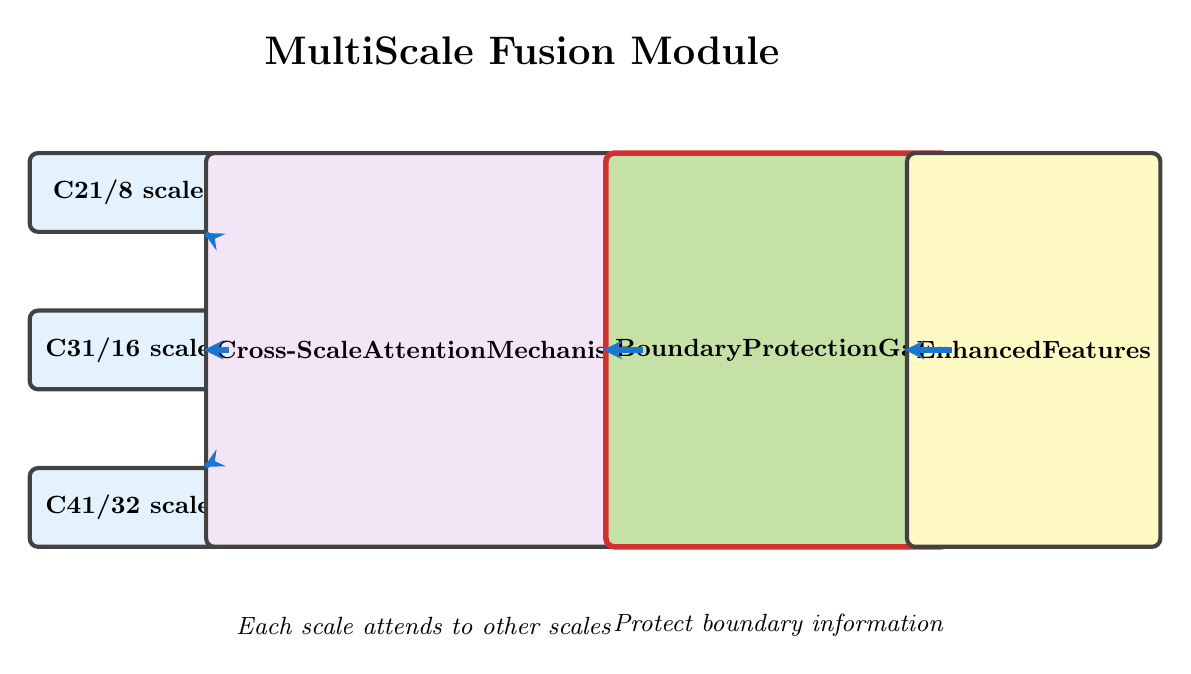
\begin{tikzpicture}[node distance=1.5cm and 2cm]
    \node[font=\Large\bfseries] (title) at (7,8.3) {MultiScale Fusion Module};
    
    % Input features
    \node[inputmodule] (c2) at (2,6.5) {C2\\1/8 scale};
    \node[inputmodule] (c3) at (2,4.5) {C3\\1/16 scale};
    \node[inputmodule] (c4) at (2,2.5) {C4\\1/32 scale};
    
    % Processing modules
    \node[fusionmodule, minimum height=5cm] (attn) at (5.75,4.5) 
          {Cross-Scale\\Attention\\Mechanism};
    \node[enhancedmodule, minimum height=5cm] (gate) at (10.25,4.5) 
          {Boundary\\Protection\\Gate};
    
    % Output
    \node[outputmodule, minimum height=5cm, minimum width=0.8cm] (out) at (13.5,4.5) 
          {Enhanced\\Features};
    
    % Arrows
    \draw[arrow] (c2) -- (attn);
    \draw[arrow] (c3) -- (attn);
    \draw[arrow] (c4) -- (attn);
    \draw[arrow] (attn) -- (gate);
    \draw[arrow] (gate) -- (out);
    
    % Annotations
    \node[font=\small\itshape] at (5.75,1) {Each scale attends to other scales};
    \node[font=\small\itshape] at (10.25,1) {Protect boundary information};
\end{tikzpicture}

% Enhanced C1C2 Fusion Module
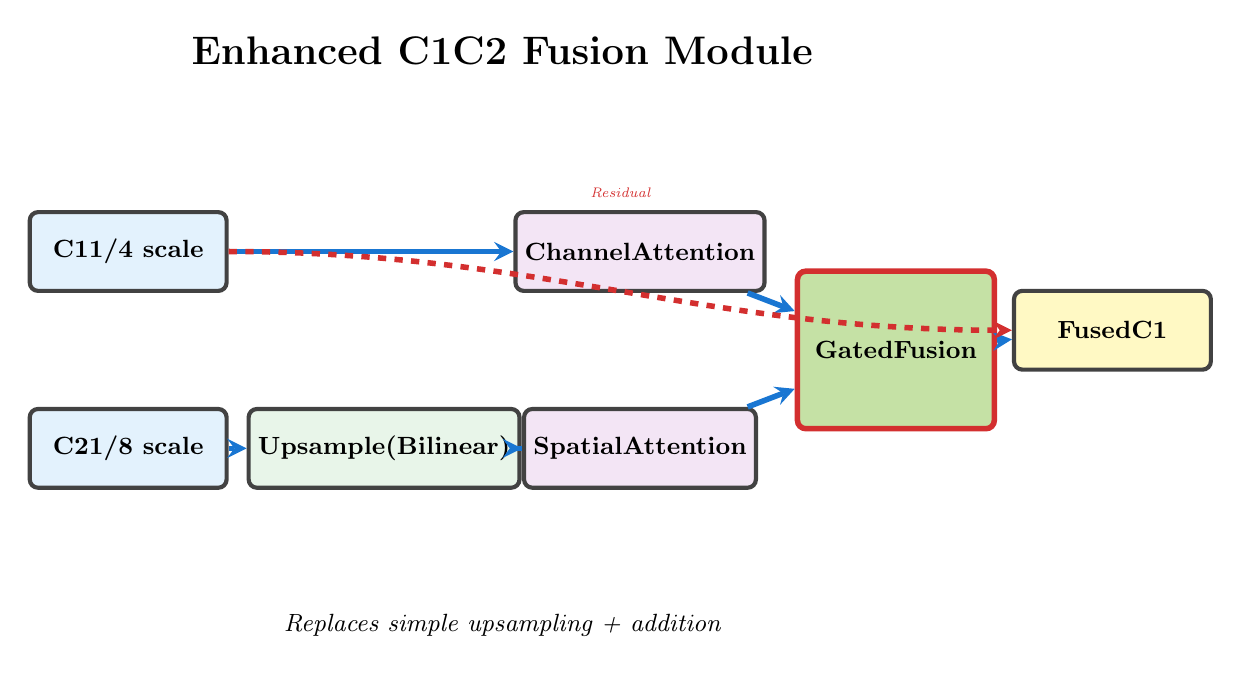
\begin{tikzpicture}[node distance=1.5cm and 2cm]
    \node[font=\Large\bfseries] (title) at (7,8.3) {Enhanced C1C2 Fusion Module};
    
    % Input
    \node[inputmodule] (c1) at (2.25,5.75) {C1\\1/4 scale};
    \node[inputmodule] (c2) at (2.25,3.25) {C2\\1/8 scale};
    
    % Upsample
    \node[adaptermodule] (upsample) at (5.5,3.25) {Upsample\\(Bilinear)};
    
    % Attention
    \node[fusionmodule] (chattn) at (8.75,5.75) {Channel\\Attention};
    \node[fusionmodule] (spattn) at (8.75,3.25) {Spatial\\Attention};
    
    % Gate
    \node[enhancedmodule, minimum height=2cm] (gate) at (12,4.5) {Gated\\Fusion};
    
    % Output
    \node[outputmodule] (out) at (14.75,4.75) {Fused\\C1};
    
    % Arrows
    \draw[arrow] (c1) -- (chattn);
    \draw[arrow] (c2) -- (upsample);
    \draw[arrow] (upsample) -- (spattn);
    \draw[arrow] (chattn) -- (gate);
    \draw[arrow] (spattn) -- (gate);
    \draw[arrow] (gate) -- (out);
    \draw[arrow, dashed, color=highlightcolor] (c1) to[out=0,in=180] (out);
    \node[font=\tiny\itshape, color=highlightcolor] at (8.5,6.5) {Residual};
    
    \node[font=\small\itshape] at (7,1) {Replaces simple upsampling + addition};
\end{tikzpicture}

% Text Attention Aggregation Module
\begin{tikzpicture}[node distance=1.5cm and 2cm]
    \node[font=\Large\bfseries] (title) at (7,8.3) {Text Attention Aggregation Module};
    
    % Input
    \node[textmodule, minimum height=2.5cm] (text) at (2.25,5.75) {Text Features\\[B$\times$N$\times$D]};
    
    % Processing
    \node[inputmodule] (base) at (5.75,6.6) {Base Token\\(EOS/CLS)};
    \node[fusionmodule] (attn) at (5.75,4.75) {Multi-Head\\Attention};
    \node[enhancedmodule] (query) at (5.75,2.25) {Learnable\\Query};
    
    % Fusion
    \node[enhancedmodule, minimum height=2.5cm] (fusion) at (9.5,4.75) {Weighted\\Fusion\\(Learnable)};
    
    % Output
    \node[outputmodule] (out) at (12.75,4.75) {Aggregated\\Text Feature};
    
    % Arrows
    \draw[arrow] (text) -- (base);
    \draw[arrow] (text) -- (attn);
    \draw[arrow] (query) -- (attn);
    \draw[arrow] (base) -- (fusion);
    \draw[arrow] (attn) -- (fusion);
    \draw[arrow] (fusion) -- (out);
    
    \node[font=\small\itshape] at (7,1) {Replaces simple token selection (EOS/CLS)};
\end{tikzpicture}

% Enhanced Loss Functions Module
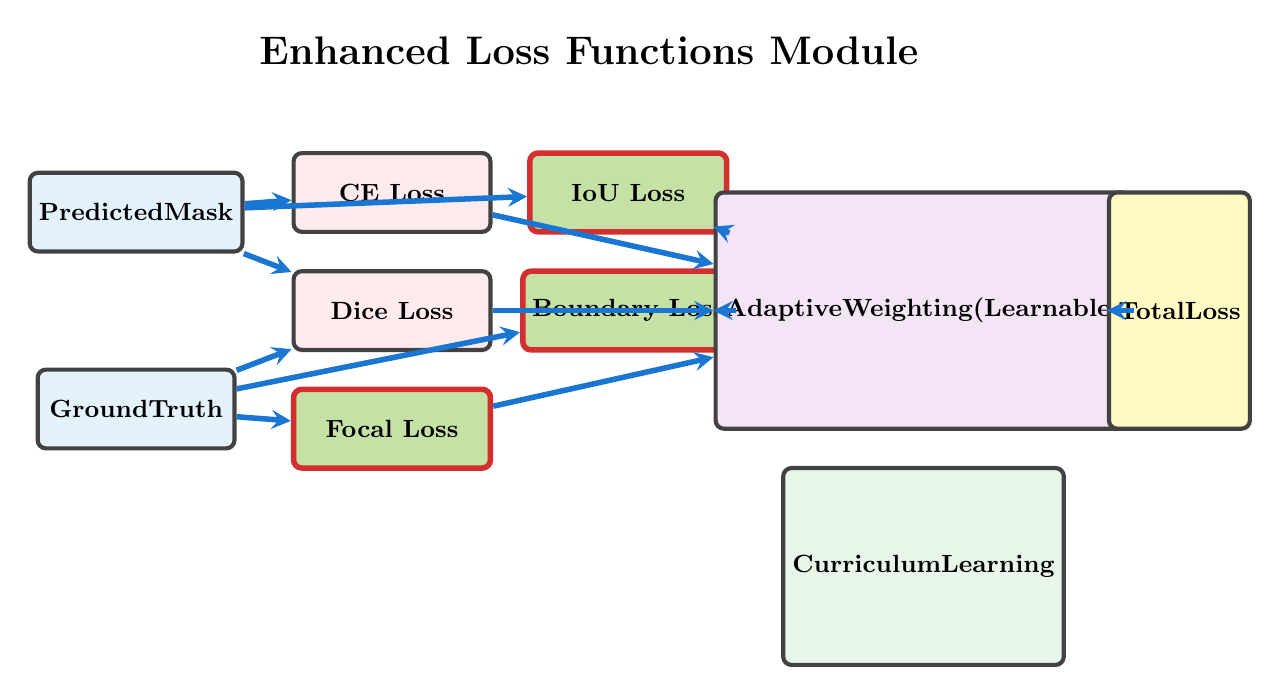
\begin{tikzpicture}[node distance=1.5cm and 2cm]
    \node[font=\Large\bfseries] (title) at (8,8.3) {Enhanced Loss Functions Module};
    
    % Input
    \node[inputmodule] (pred) at (2.25,6.25) {Predicted\\Mask};
    \node[inputmodule] (target) at (2.25,3.75) {Ground\\Truth};
    
    % Loss functions
    \node[lossmodule] (ce) at (5.5,6.5) {CE Loss};
    \node[lossmodule] (dice) at (5.5,5) {Dice Loss};
    \node[enhancedmodule] (focal) at (5.5,3.5) {Focal Loss};
    \node[enhancedmodule] (iou) at (8.5,6.5) {IoU Loss};
    \node[enhancedmodule] (boundary) at (8.5,5) {Boundary Loss};
    
    % Adaptive weighting
    \node[fusionmodule, minimum height=3cm] (adaptive) at (12.25,5) {Adaptive\\Weighting\\(Learnable)};
    
    % Curriculum learning
    \node[adaptermodule, minimum height=2.5cm] (curriculum) at (12.25,1.75) {Curriculum\\Learning};
    
    % Total loss
    \node[outputmodule, minimum height=3cm, minimum width=1cm] (total) at (15.5,5) {Total\\Loss};
    
    % Arrows
    \draw[arrow] (pred) -- (ce);
    \draw[arrow] (pred) -- (dice);
    \draw[arrow] (target) -- (focal);
    \draw[arrow] (target) -- (dice);
    \draw[arrow] (pred) -- (iou);
    \draw[arrow] (target) -- (boundary);
    \draw[arrow] (ce) -- (adaptive);
    \draw[arrow] (dice) -- (adaptive);
    \draw[arrow] (focal) -- (adaptive);
    \draw[arrow] (iou) -- (adaptive);
    \draw[arrow] (boundary) -- (adaptive);
    \draw[arrow] (adaptive) -- (total);
\end{tikzpicture}

\end{document}


% Requires: \usepackage{tikz} \usetikzlibrary{shapes,arrows,positioning,calc}

\documentclass[tikz,border=2mm]{standalone}
\usepackage{tikz}
\usetikzlibrary{shapes,arrows,positioning,calc,decorations.pathreplacing}

% Color definitions (professional scheme)
\definecolor{inputcolor}{RGB}{227,242,253}
\definecolor{encodercolor}{RGB}{255,243,224}
\definecolor{adaptercolor}{RGB}{232,245,233}
\definecolor{fusioncolor}{RGB}{243,229,245}
\definecolor{decodercolor}{RGB}{252,228,236}
\definecolor{outputcolor}{RGB}{255,249,196}
\definecolor{losscolor}{RGB}{255,235,238}
\definecolor{textcolor}{RGB}{224,242,241}
\definecolor{enhancedcolor}{RGB}{197,225,165}
\definecolor{bordercolor}{RGB}{66,66,66}
\definecolor{arrowcolor}{RGB}{25,118,210}
\definecolor{highlightcolor}{RGB}{211,47,47}

\tikzset{
    module/.style={
        rectangle,
        rounded corners=3pt,
        minimum width=2.5cm,
        minimum height=1cm,
        text centered,
        draw=bordercolor,
        line width=1.5pt,
        font=\small\bfseries
    },
    inputmodule/.style={module, fill=inputcolor},
    encodermodule/.style={module, fill=encodercolor},
    adaptermodule/.style={module, fill=adaptercolor},
    fusionmodule/.style={module, fill=fusioncolor},
    decodermodule/.style={module, fill=decodercolor},
    outputmodule/.style={module, fill=outputcolor},
    lossmodule/.style={module, fill=losscolor},
    textmodule/.style={module, fill=textcolor},
    enhancedmodule/.style={module, fill=enhancedcolor, draw=highlightcolor, line width=2pt},
    arrow/.style={->, >=stealth, line width=2pt, color=arrowcolor}
}

\begin{document}

% Overall Architecture
\begin{tikzpicture}[node distance=1.5cm and 2cm]
    % Title
    \node[font=\Large\bfseries] (title) at (9,10.5) {Enhanced ReferSAM Architecture};
    
    % Input layer
    \node[inputmodule] (image) at (2.25,9) {Image\\[B$\times$3$\times$H$\times$W]};
    \node[textmodule] (text) at (2.25,7.3) {Text\\[B$\times$N]};
    
    % Encoders
    \node[encodermodule] (vit) at (5.75,9) {ViT Image\\Encoder};
    \node[encodermodule] (textenc) at (5.75,7.3) {Text\\Encoder};
    
    % ViT Adapter (main container)
    \node[adaptermodule, minimum width=4.5cm, minimum height=3.5cm, 
          fill=adaptercolor!30, draw=bordercolor, line width=2pt] (adapter) at (10.25,7.5) {};
    \node[font=\large\bfseries] (adaptertitle) at (10.25,9.2) {ViT Adapter (Enhanced)};
    
    % Enhanced modules inside adapter
    \node[enhancedmodule, minimum width=3.5cm, minimum height=0.8cm] 
          (msf) at (10.25,8.4) {MultiScale Fusion};
    \node[enhancedmodule, minimum width=3.5cm, minimum height=0.8cm] 
          (c1c2) at (10.25,7.4) {Enhanced C1C2 Fusion};
    \node[enhancedmodule, minimum width=3.5cm, minimum height=0.8cm] 
          (textattn) at (10.25,6.4) {Text Attention Aggregation};
    
    % Features
    \node[adaptermodule] (feat) at (14.75,7.6) {Adapter\\Features};
    \node[decodermodule] (maskfeat) at (14.75,5.8) {Mask Feature\\\& Prompts};
    \node[decodermodule] (decoder) at (14.75,3.5) {SAM Mask\\Decoder};
    \node[outputmodule] (output) at (14.75,1.5) {Predicted\\Mask};
    
    % Loss
    \node[lossmodule, minimum height=2cm, draw=highlightcolor, line width=2pt] 
          (loss) at (2.5,4) {Enhanced Loss\\Functions\\(Focal+IoU+Boundary)};
    
    % Arrows
    \draw[arrow] (image) -- (vit);
    \draw[arrow] (text) -- (textenc);
    \draw[arrow] (vit) -- (adapter);
    \draw[arrow] (textenc) -- (adapter);
    \draw[arrow] (adapter) -- (feat);
    \draw[arrow] (feat) -- (maskfeat);
    \draw[arrow] (maskfeat) -- (decoder);
    \draw[arrow] (decoder) -- (output);
    \draw[arrow, dashed, color=highlightcolor] (output) to[out=180,in=0] (loss);
    \node[font=\small\itshape, color=highlightcolor] at (8.5,1.5) {Training Loss};
\end{tikzpicture}

% MultiScale Fusion Module
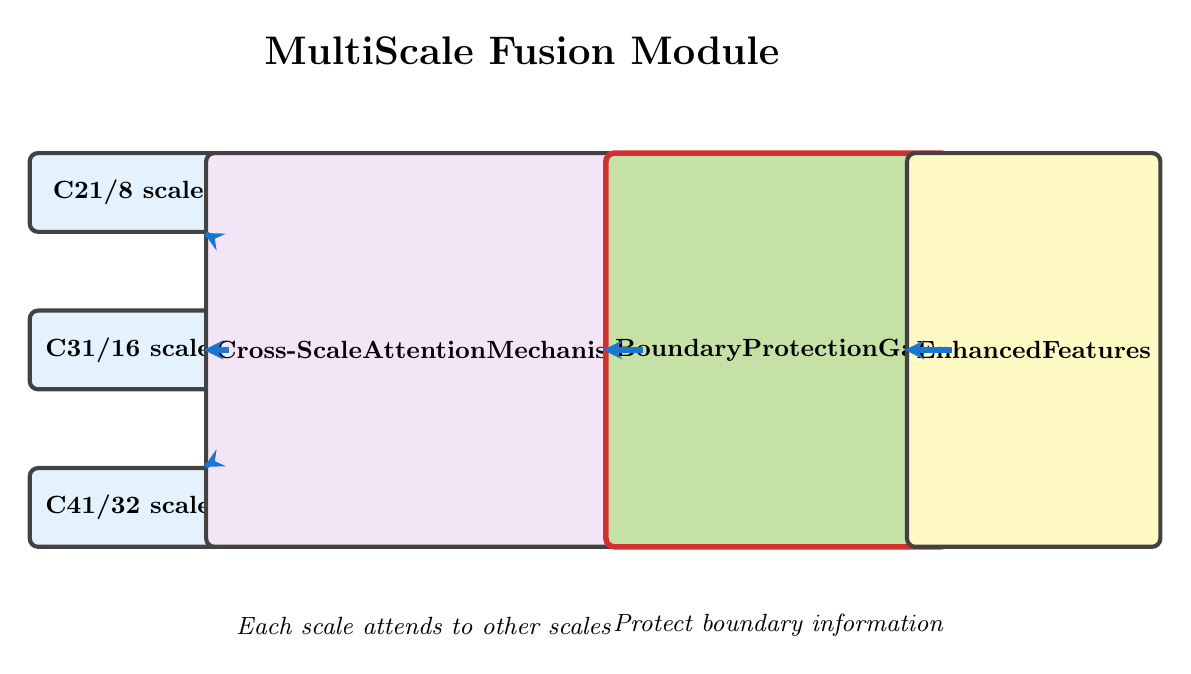
\begin{tikzpicture}[node distance=1.5cm and 2cm]
    \node[font=\Large\bfseries] (title) at (7,8.3) {MultiScale Fusion Module};
    
    % Input features
    \node[inputmodule] (c2) at (2,6.5) {C2\\1/8 scale};
    \node[inputmodule] (c3) at (2,4.5) {C3\\1/16 scale};
    \node[inputmodule] (c4) at (2,2.5) {C4\\1/32 scale};
    
    % Processing modules
    \node[fusionmodule, minimum height=5cm] (attn) at (5.75,4.5) 
          {Cross-Scale\\Attention\\Mechanism};
    \node[enhancedmodule, minimum height=5cm] (gate) at (10.25,4.5) 
          {Boundary\\Protection\\Gate};
    
    % Output
    \node[outputmodule, minimum height=5cm, minimum width=0.8cm] (out) at (13.5,4.5) 
          {Enhanced\\Features};
    
    % Arrows
    \draw[arrow] (c2) -- (attn);
    \draw[arrow] (c3) -- (attn);
    \draw[arrow] (c4) -- (attn);
    \draw[arrow] (attn) -- (gate);
    \draw[arrow] (gate) -- (out);
    
    % Annotations
    \node[font=\small\itshape] at (5.75,1) {Each scale attends to other scales};
    \node[font=\small\itshape] at (10.25,1) {Protect boundary information};
\end{tikzpicture}

% Enhanced C1C2 Fusion Module
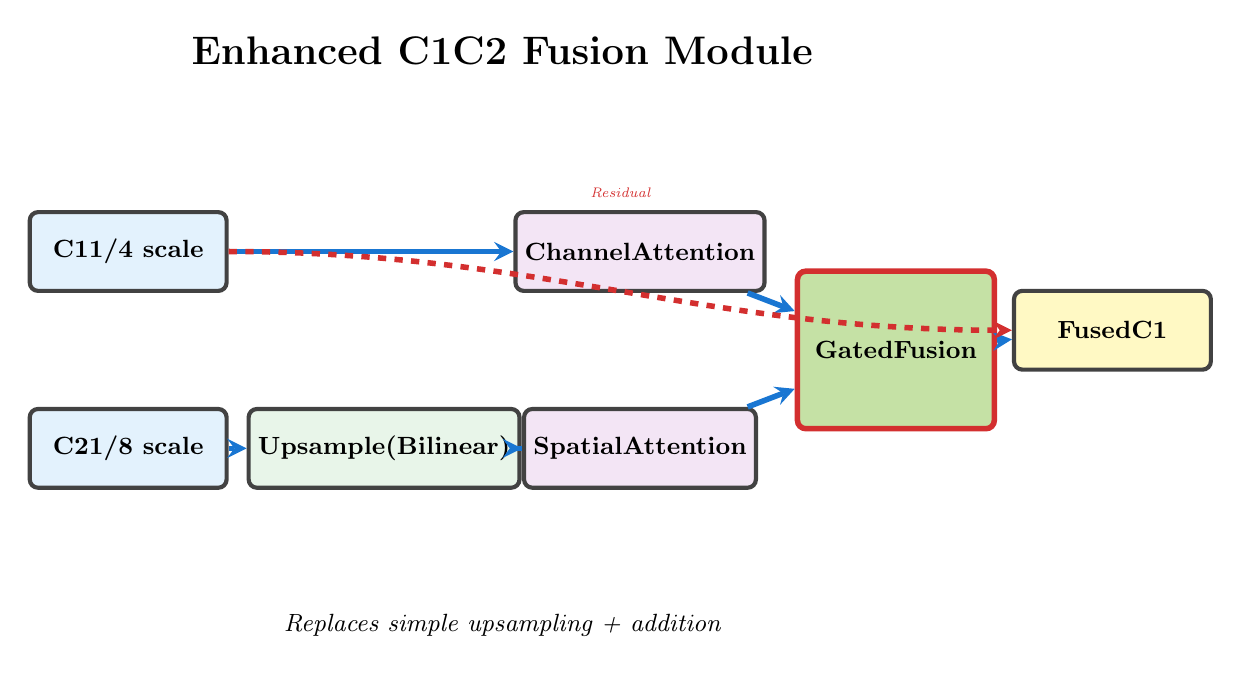
\begin{tikzpicture}[node distance=1.5cm and 2cm]
    \node[font=\Large\bfseries] (title) at (7,8.3) {Enhanced C1C2 Fusion Module};
    
    % Input
    \node[inputmodule] (c1) at (2.25,5.75) {C1\\1/4 scale};
    \node[inputmodule] (c2) at (2.25,3.25) {C2\\1/8 scale};
    
    % Upsample
    \node[adaptermodule] (upsample) at (5.5,3.25) {Upsample\\(Bilinear)};
    
    % Attention
    \node[fusionmodule] (chattn) at (8.75,5.75) {Channel\\Attention};
    \node[fusionmodule] (spattn) at (8.75,3.25) {Spatial\\Attention};
    
    % Gate
    \node[enhancedmodule, minimum height=2cm] (gate) at (12,4.5) {Gated\\Fusion};
    
    % Output
    \node[outputmodule] (out) at (14.75,4.75) {Fused\\C1};
    
    % Arrows
    \draw[arrow] (c1) -- (chattn);
    \draw[arrow] (c2) -- (upsample);
    \draw[arrow] (upsample) -- (spattn);
    \draw[arrow] (chattn) -- (gate);
    \draw[arrow] (spattn) -- (gate);
    \draw[arrow] (gate) -- (out);
    \draw[arrow, dashed, color=highlightcolor] (c1) to[out=0,in=180] (out);
    \node[font=\tiny\itshape, color=highlightcolor] at (8.5,6.5) {Residual};
    
    \node[font=\small\itshape] at (7,1) {Replaces simple upsampling + addition};
\end{tikzpicture}

% Text Attention Aggregation Module
\begin{tikzpicture}[node distance=1.5cm and 2cm]
    \node[font=\Large\bfseries] (title) at (7,8.3) {Text Attention Aggregation Module};
    
    % Input
    \node[textmodule, minimum height=2.5cm] (text) at (2.25,5.75) {Text Features\\[B$\times$N$\times$D]};
    
    % Processing
    \node[inputmodule] (base) at (5.75,6.6) {Base Token\\(EOS/CLS)};
    \node[fusionmodule] (attn) at (5.75,4.75) {Multi-Head\\Attention};
    \node[enhancedmodule] (query) at (5.75,2.25) {Learnable\\Query};
    
    % Fusion
    \node[enhancedmodule, minimum height=2.5cm] (fusion) at (9.5,4.75) {Weighted\\Fusion\\(Learnable)};
    
    % Output
    \node[outputmodule] (out) at (12.75,4.75) {Aggregated\\Text Feature};
    
    % Arrows
    \draw[arrow] (text) -- (base);
    \draw[arrow] (text) -- (attn);
    \draw[arrow] (query) -- (attn);
    \draw[arrow] (base) -- (fusion);
    \draw[arrow] (attn) -- (fusion);
    \draw[arrow] (fusion) -- (out);
    
    \node[font=\small\itshape] at (7,1) {Replaces simple token selection (EOS/CLS)};
\end{tikzpicture}

% Enhanced Loss Functions Module
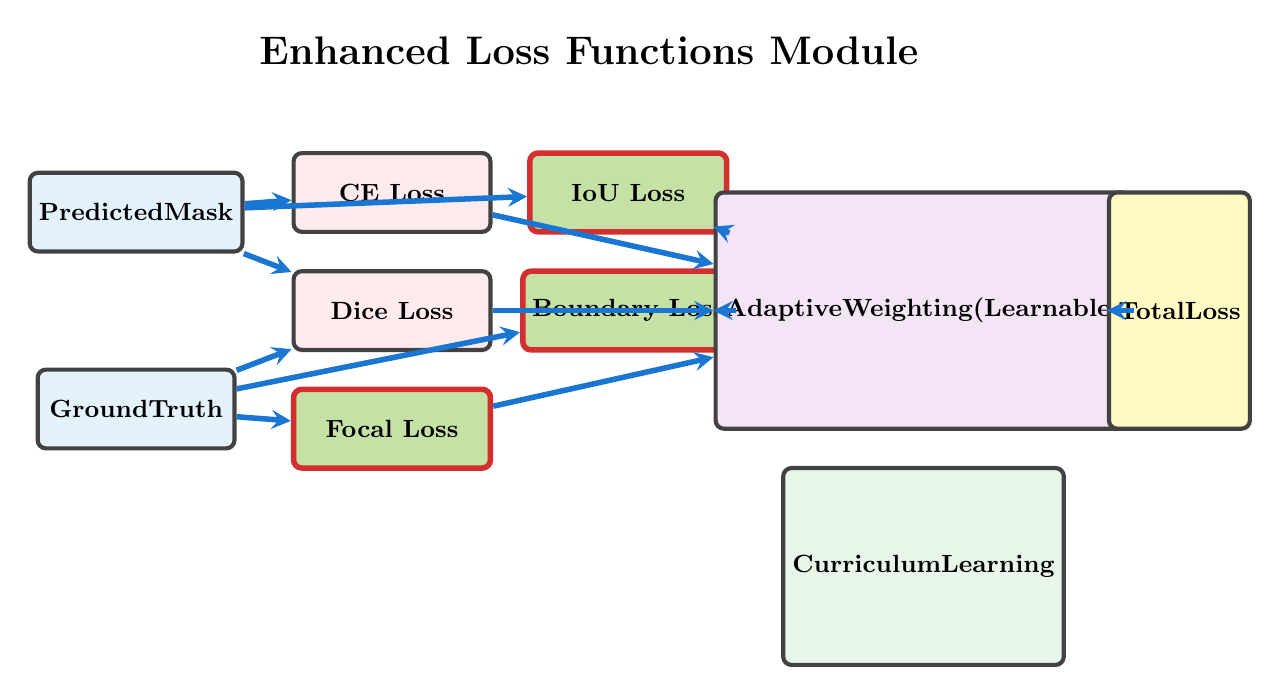
\begin{tikzpicture}[node distance=1.5cm and 2cm]
    \node[font=\Large\bfseries] (title) at (8,8.3) {Enhanced Loss Functions Module};
    
    % Input
    \node[inputmodule] (pred) at (2.25,6.25) {Predicted\\Mask};
    \node[inputmodule] (target) at (2.25,3.75) {Ground\\Truth};
    
    % Loss functions
    \node[lossmodule] (ce) at (5.5,6.5) {CE Loss};
    \node[lossmodule] (dice) at (5.5,5) {Dice Loss};
    \node[enhancedmodule] (focal) at (5.5,3.5) {Focal Loss};
    \node[enhancedmodule] (iou) at (8.5,6.5) {IoU Loss};
    \node[enhancedmodule] (boundary) at (8.5,5) {Boundary Loss};
    
    % Adaptive weighting
    \node[fusionmodule, minimum height=3cm] (adaptive) at (12.25,5) {Adaptive\\Weighting\\(Learnable)};
    
    % Curriculum learning
    \node[adaptermodule, minimum height=2.5cm] (curriculum) at (12.25,1.75) {Curriculum\\Learning};
    
    % Total loss
    \node[outputmodule, minimum height=3cm, minimum width=1cm] (total) at (15.5,5) {Total\\Loss};
    
    % Arrows
    \draw[arrow] (pred) -- (ce);
    \draw[arrow] (pred) -- (dice);
    \draw[arrow] (target) -- (focal);
    \draw[arrow] (target) -- (dice);
    \draw[arrow] (pred) -- (iou);
    \draw[arrow] (target) -- (boundary);
    \draw[arrow] (ce) -- (adaptive);
    \draw[arrow] (dice) -- (adaptive);
    \draw[arrow] (focal) -- (adaptive);
    \draw[arrow] (iou) -- (adaptive);
    \draw[arrow] (boundary) -- (adaptive);
    \draw[arrow] (adaptive) -- (total);
\end{tikzpicture}

\end{document}

